\documentclass[a4paper,12pt]{article}

\usepackage[utf8]{inputenc}   % Codificação UTF-8
\usepackage[T1]{fontenc}      % Codificação da fonte
\usepackage{enumitem}
\usepackage{graphicx}
\usepackage{caption}
\usepackage{float}
\usepackage{pgffor}

\newcommand\Insert[1]{%
    \foreach \x in {#1}{%
        \begin{figure}[H]
            \centering
            \includegraphics[width=0.6\textwidth]{Aula03/Daniel/\x.png} % adjust path
            \caption*{\x} % <- custom caption (no "Figure" label, no numbering)
            \label{fig:Graphic\x} % still works for \ref if you want
        \end{figure}
    }%
}


\title{LFTC}
\author{Miguel de Campos R. Moret \\ Abigail Sayury Nakashima}
\date{\today}

\begin{document}

\maketitle
\newpage

\tableofcontents
\newpage

\section{Aula 02 }
    \subsection{Descreva as linguagens denotadas pelas ER’s abaixo sobre o alfabeto $\sum = \{0,1\}$.}
    \begin{enumerate}[label=\textbf{\alph* -}]
        \item $\mathbf{0|10^*}$
            \\ A linguagem é composta por cadeias que contêm apenas o símbolo $0$ ou que iniciam com $1$ seguido de qualquer quantidade (inclusive zero) de $0$'s.
        \item $\mathbf{(0|1)0^*}$
            \\ A linguagem é composta por cadeias que iniciam com $0$ ou com $1$ e são seguidos por qualquer quantidade (inclusive zero) de $0$'s.
        \item $\mathbf{(0011)^*}$
            \\ A linguagem é composta por cadeias compostas por qualquer quan\-tidade (inclusive zero) da substring "$0011$".
        \item $\mathbf{(0|1)^*1(0|1)^*}$
            \\ A linguagem é composta por cadeias que contem pelo menos um $1$.
        \item $\mathbf{0^*11^*0}$
            \\ A linguagem é composta por cadeias que iniciam com qualquer quan\-tidade (inclusive zero) de $0$'s, segiodos por pelo menos um $1$, finalizando com um único símbolo $0$.
        \item $\mathbf{0(0|1)^*0}$
            \\ A linguagem é composta por cadeias que iniciam e  terminam com $0$.
        \item $\mathbf{(\epsilon+0)(\epsilon|1)}$
            \\ A linguagem é composta por 4 cadeias diferentes: uma cadeia sem símbolos ("vazia"), uma cadeia composta por um único $0$, uma cadeia composta por um único $1$ e uma cadeia composta por um $0$ seguido por um $1$.
        \item $\mathbf{(000^*|1)^*}$
            \\ A linguagem é composta por cadeias que não contêm $0$'s sozinhos (eles estão sempre em grupos de $2+$).
        \item $\mathbf{(0^*|0^*11(1|00^*11)^*)(\epsilon|00^*)}$
            \\ A linguagem de todas as cadeias em que cada bloco de 1’s tem comprimento pelo menos 2.
    \end{enumerate}

    \subsection{Sobre o $\sum = \{a,b\}$, defina expressoes regulares que representam as linguagens cujas sentencas estao descritas a seguir} 
    \begin{itemize}
        \item \textbf{Possuem comprimento maior ou igual a 3;}
            \\ $(a|b)(a|b)(a|b)(a|b)*$
        \item \textbf{Possuem comprimento menor ou igual a 3;}
            \\ $*(a|b|\epsilon)(a|b|\epsilon)(a|b|\epsilon)$
        \item \textbf{Possuem comprimento diferente a 3;}
            \\ $((a|b|\epsilon)(a|b|\epsilon))|((a|b)(a|b)(a|b)(a|b)*)$
        \item \textbf{Possuem comprimento par;}
            \\ $((a|b)(a|b))^*$
        \item \textbf{Possuem comprimento impar;}
            \\ $(a|b)((a|b)(a|b))^*$
        \item \textbf{Possuem comprimento multiplo de 4;}
            \\ $(a|b)(a|b)(a|b)(a|b)((a|b)(a|b)(a|b)(a|b))^*$
    \end{itemize}

    \subsection{Fazer o conjunto de exercícios da seção 3.1 do livro do HOPCROFT, páginas 96 e 97.} 
        \subsubsection{Escreva expressões regulares corresponden\-tes às seguintes linguagens:}
            \begin{enumerate}[label={\bfseries \alph*)}]
                \item O conjunto de strings sobre o alfabeto $\{a, b, c\}$ que contém pelo menos um $a$ e um $b$.
                    \\ $((c|a|b)^* a(c|a|b)^* b(c|a|b)^*)|((c|a|b)^* b(c|a|b)^* a(c|a|b)^*)$.
                \item O conjunto de strings $0$'s e $1$'s cujo décimo símbolo a partir da extremidade direita é $1$.
                    \\ $(0|1)^* 1 (0|1)(0|1)(0|1)(0|1)(0|1)(0|1)(0|1)(0|1)(0|1)$.
                \item O conjunto de strings $0$'s e $1$'s com no máximo um par de $1$'s consecutivos.
                    \\ $(0|10)^*(11)?(0|01)^*$
            \end{enumerate}
            
        \subsubsection{Escreva expressões regulares corresponden\-tes às seguintes linguagens:}
            \begin{enumerate}[label={\bfseries \alph*)}]
                \item O conjunto de todos os strings de $0$'s e $1$'s tais que todo par de $0$'s adjacentes aparece antes de qualquer par de $1$'s adjacentes.
                    \\ $(1^*(01)^*)^*(00)^*(0^*(10)^*)^*(11)^*(1^*(01)^*)^*$
                \item O conjunto de strings $0$'s e $1$'s cujo número de $0$'s é divisível por $5$.
                    \\ $(1^*01^*01^*01^*01^*0)(1^*01^*01^*01^*01^*0)^*$
            \end{enumerate}
        
        \subsubsection{Escreva expressões regulares corresponden\-tes às seguintes linguagens:}
            \begin{enumerate}[start=1, label={\bfseries \alph*)}]
                \item O conjunto de todos os strings $0$'s e $1$'s que não contêm $101$ como um substring.
                    \\ $(0^*|1^*)(0^*|1^*)(0^*00(1^*)|0^*)^*$
                \item O conjunto de todos os strings com um número igual de $0$'s e $1$'s, tais que nenhum prefixo tenha dois $0$'s a mais que os $1$'s, nem dois $1$'s a mais que os $0$'s.
                    \\ $(01|10|0011|1100|1001|0110)*$
                \item O conjunto de strings de $0$'s e $1$'scujo número de $0$'s é divisível por $5$ e cujo número de $1$'s é par.
                    \\ $((11)^*0(11)^*0(11)^*0(11)^*0(11)^*0)((11)^*0(11)^*0(11)^*0(11)^*0(11)^*0)^*$
            \end{enumerate}
        
            \subsubsection{Forneça descrições em português das linguagens correspon\-dedentes às seguintes expressões regulares:}
            \begin{enumerate}[label={\bfseries \alph*)}]
                \item $\mathbf{(1+\epsilon)(00^*)^*0^*}$.
                    \\ Linguagem de todas as cadeias com $\sum=\{0,1\}$ que são ou vazias, ou contém somente zeros, ou possuem um único $1$ seguido por múltiplos (ou nenhum) $0$'s.
                \item $\mathbf{(0^*1^*)^*000(0+1)^*}$.
                    \\ Linguagem de todas as cadeias com $\sum=\{0,1\}$ que contêm “000” como substring.
                \item $\mathbf{(0+10)^*1^*}$.
                    \\ Linguagem de todas as cadeias com $\sum=\{0,1\}$ que contêm pares $11$ somente no final da cadeia.
            \end{enumerate}

            \subsubsection{No Exemplo 3.1, destacamos que $\emptyset$ é uma das duas linguagens cujo fechammento é finito. Qual é a outra?}
                A outra linguagem é $\mathbf{\epsilon}$

\section{Aula 03 - Feito junto de Daniel Padua}

    \foreach \i in {1,...,11}{
    \begin{figure}[H] 
        \centering
        \includegraphics[width=0.5\textwidth]{Aula03/Daniel/\i.png}
        \caption*{\i}
    \end{figure}
    }
    \foreach \i in {15,...,19}{
    \begin{figure}[H] 
        \centering
        \includegraphics[width=0.5\textwidth]{Aula03/Daniel/\i.png}
        \caption*{\i}
    \end{figure}
    }
    \foreach \i in {20,...,29}{
    \begin{figure}[H]
        \centering
        \includegraphics[width=0.5\textwidth]{Aula03/Abigail/\i.png}
        \caption*{\i}
    \end{figure}
    }

\begin{enumerate}
    \item[30)] 
    $G = (\{S,A\}, \{a,b,c\}, P, S)$, com \\
    $P = \{ S \to aS \mid bA \mid cS \mid \epsilon,\;
    A \to aA \mid bS \mid cA \}$ \\[6pt]
    ER: $((a|c)*((a|c)*b(a|c)*b)*)*$

    \item[31)] 
    $G = (\{S,A\}, \{a,b,c\}, P, S)$, com \\
    $P = \{ S \to aS \mid bS \mid cA \mid c,\;
    A \to aA \mid bA \mid cS \mid \epsilon \}$ \\[6pt]
    ER: $[ab]*c([ab]*c[ab]*c)*[ab]*$

    \item[32)] 
    $G = (\{S,A,B,C\}, \{a,b,c\}, P, S)$, com \\
    $P = \{ 
    S \to aB \mid bS \mid cA,\;
    A \to aC \mid bA \mid cS \mid \epsilon,\;
    B \to aS \mid bB \mid cC,\;
    C \to aA \mid bC \mid cB \}$ \\[6pt]
    ER: $(b*(ab*ab*)*cb*(ab*ab*)*) \mid (b*(ab*ab*)*ab*cb*(ab*ab*)*ab*)(c[(b*(ab*ab*)*cb*(ab*ab*)*) \mid (b*(ab*ab*)*ab*cb*(ab*ab*)*ab*)])* $

    \item[33)] 
    $G = (\{S,A\}, \{a,b,c\}, P, S)$, com \\
    $P = \{ 
    S \to aS \mid bS \mid cS \mid abcA,\;
    A \to \epsilon \}$ \\[6pt]
    ER: $[ac]*abc[ac]*$

    \item[34)] 
    $G = (\{S,A,B,C,D\}, \{a,b,c\}, P, S)$, com \\
    $P = \{ 
    S \to aS \mid bS \mid cS \mid aA \mid bB \mid cC,\;
    A \to aaS \mid aaD,\;
    B \to bbS \mid bbD,\;
    C \to ccS \mid ccD,\;
    D \to aD \mid bD \mid cD \mid \epsilon \}$ \\[6pt]
    ER: $[ac]*(aaa \mid bbb \mid ccc)[ac]*$

    \item[35)] 
    $G = (\{S,A,B,C\}, \{a,b,c\}, P, S)$, com \\
    $P = \{ 
    S \to A \mid B \mid C \mid \epsilon,\;
    A \to bB \mid CC \mid \epsilon,\;
    B \to aA \mid cC \mid \epsilon,\;
    C \to bB \mid cC \mid \epsilon \}$ \\[6pt]
    ER: $(a(b|c) \mid b(a|c) \mid c(a|b))*$

    \item[36)] 
    $G = (\{S\}, \{a,b,c\}, P, S)$, com \\
    $P = \{ S \to bS \mid cS \mid \epsilon \}$ \\[6pt]
    ER: $(b|c|a(a|c)?)*$

    \item[37)] 
    $G = (\{S,A\}, \{a,b,c\}, P, S)$, com \\
    $P = \{ 
    S \to aA \mid bS \mid cS \mid \epsilon,\;
    A \to aA \mid cS \mid \epsilon \}$ \\[6pt]
    ER: $(b|c|a(b|a|c)?)*$

    \item[38)] 
    $G = (\{S,A\}, \{a,b,c\}, P, S)$, com \\
    $P = \{ 
    S \to aA \mid bS \mid cS \mid \epsilon,\;
    A \to aA \mid bB \mid cS \mid \epsilon,\;
    B \to aA \mid bS \mid \ epsilon \}$ \\[6pt]
    ER: $(b|c|a(b|a|c)?)*$
\end{enumerate}

\section{Aula 04}
    \foreach \i in {1,...,18}{
    \begin{figure}[H]
        \centering
        \includegraphics[width=0.5\textwidth]{Aula04/\i.png}
        \caption*{\i}
    \end{figure}
    }

\section{Aula 07}
    \subsection{Exercício 5}
        \begin{figure}[H]
            \centering
            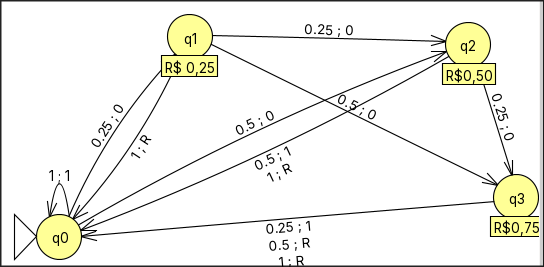
\includegraphics[width=0.8\textwidth]{Aula07/Images/Exercicio1.png}
            \caption*{1}
        \end{figure}
        Diagrama de Estados:
        \begin{itemize}
            \item q0 (estado inicial)
                \begin{itemize}
                    \item $0.25 \to q1 | S = 0$
                    \item $0.50 \to q2 | S = 0$
                    \item $1.00 \to q0 | S = 1$
                \end{itemize}
            \item q1
                \begin{itemize}
                    \item $0.25 \to q2 | S = 0$
                    \item $0.50 \to q0 | S = 1$
                    \item $1.00 \to q0 | S = R$
                \end{itemize}
            \item q2
                \begin{itemize}
                    \item $0.25 \to q3 | S = 0$
                    \item $0.50 \to q0 | S = 1$
                    \item $1.00 \to q0 | S = R$
                \end{itemize}
            \item q3
                \begin{itemize}
                    \item $0.25 \to q0 | S = 1$
                    \item $0.50 \to q0 | S = R$
                    \item $1.00 \to q0 | S = R$
                \end{itemize}                
        \end{itemize}
    
    \subsection{Exercício 6}
        \begin{figure}[H]
            \centering
            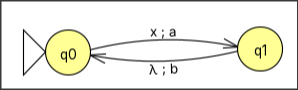
\includegraphics[width=0.8\textwidth]{Aula07/Images/Exercicio2.png}
            \caption*{1}
        \end{figure}

        \[AF = (\{Parado, Subindo, Descendo\}, \{=, >, <\}, \{Parar, Subir, Descer\}, \delta, \gamma, q0)\]
        
        \begin{itemize}
            \item Função de transição ($\delta$):
                \begin{center}
                    \begin{tabular}{|c|c|c|}
                        \hline
                        Estado Atual & Condição & Próximo Estado | Saída \\
                        \hline
                        $q_0$ & requisitado $=$ atual & $q_0 \,|\, S = Parar$ \\
                        \hline
                        $q_1$ & requisitado $=$ atual & $q_0 \,|\, S = Parar$ \\
                        \hline  
                    \end{tabular}
                \end{center}
                
            \item Função Saída ($\gamma$):
            \begin{center}
                \begin{tabular}{|c|c|c|}
                    \hline
                    Estado Atual & Entrada & Saída\\
                    \hline
                    $q_0$ & $x$ & $a\\
                    \hline
                    $q_1$ & Subir\\
                    \hline
                    Descendo & Descer\\
                    \hline
                \end{tabular}
            \end{center}
        \end{itemize}

        Diagrama de Estados:
        \begin{itemize}
            \item q0 (estado inicial)
                \begin{itemize}
                    \item $x \to q1 | S = a$
                \end{itemize}
            \item q1
                \begin{itemize}
                    \item $\lambda \to q0 | S = b$
                \end{itemize}
        \end{itemize}

    \subsection{Exercício 7}
        \begin{figure}[H]
            \centering
            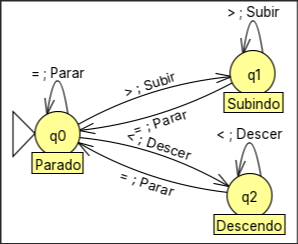
\includegraphics[width=0.8\textwidth]{Aula07/Images/Exercicio7.png}
            \caption*{7}
        \end{figure}
        
        \[AF = (\{Parado, Subindo, Descendo\}, \{=, >, <\}, \{Parar, Subir, Descer\}, \delta, \gamma, q0)\]
        
        \begin{itemize}
            \item Função de transição ($\delta$):
                \begin{center}
                    \begin{tabular}{|c|c|c|}
                        \hline
                        Estado Atual & Condição & Próximo Estado | Saída \\
                        \hline
                        $q_0$ & requisitado $=$ atual & $q_0 \,|\, S = Parar$ \\
                        $q_0$ & requisitado $>$ atual & $q_1 \,|\, S = Subir$ \\
                        $q_0$ & requisitado $<$ atual & $q_2 \,|\, S = Descer$ \\
                        \hline
                        $q_1$ & requisitado $=$ atual & $q_0 \,|\, S = Parar$ \\
                        $q_1$ & requisitado $>$ atual & $q_1 \,|\, S = Subir$ \\
                        \hline
                        $q_2$ & requisitado $=$ atual & $q_0 \,|\, S = Parar$ \\
                        $q_2$ & requisitado $<$ atual & $q_2 \,|\, S = Descer$ \\
                        \hline  
                    \end{tabular}
                \end{center}
                
            \item Função Saída ($\gamma$):
            \begin{center}
                \begin{tabular}{|c|c|}
                    \hline
                    Parado & Parar\\
                    \hline
                    Subindo & Subir\\
                    \hline
                    Descendo & Descer\\
                    \hline
                \end{tabular}
            \end{center}
        \end{itemize}



\end{document}